\documentclass[11pt]{article}
\usepackage{graphicx}
\usepackage{fancyhdr}
\usepackage{wrapfig}
\usepackage{hyperref}
\usepackage{tabularx}
\usepackage{setspace}
\usepackage[spanish]{babel}

\newsavebox\CBox
\def\textBF#1{\sbox\CBox{#1}\resizebox{\wd\CBox}{\ht\CBox}{\textbf{#1}}}

\newenvironment{myenv}[1]
  {\begin{spacing}{#1}}
  {\end{spacing}}

\addtolength{\textwidth}{0.2cm}
\setlength{\parskip}{13pt}
\setlength{\parindent}{0.0cm}
\linespread{1.25}

\pagestyle{fancy}
\fancyhf{}
\rhead{TP - Cipullo, Sullivan}
\lhead{Probalidad y Estad\'istica}
\rfoot{\vspace{1cm} \thepage}

\renewcommand*\contentsname{\LARGE Índice}

\begin{document}

\begin{titlepage}
    \begin{center}
        \vfill
        \vfill
            \vspace{0.7cm}
            \noindent\textbf{\Huge Trabajo Pr\'actico}\par
            \noindent\textbf{\Huge Estad\'istica Descriptiva}\par
            \vspace{.5cm}
        \vfill
        \noindent \textbf{\huge Alumnas:}\par
        \vspace{.5cm}
        \noindent \textbf{\Large Cipullo, In\'es}\par
        \noindent \textbf{\Large Sullivan, Katherine}\par
 
        \vfill
        \large Universidad Nacional de Rosario \par
        \noindent\large 2021
    \end{center}
\end{titlepage}
\par

El presente informe tiene como objetivo la exposici\'on de un an\'alisis estad\'istico descriptivo
sobre los datos recopilados del sistema de bicicletas compartidas de la Ciudad de Buenos Aires, EcoBici.

\section{Sobre los datos}
Los datos utilizados se encontraban divididos en dos unidades de an\'alisis diferentes: una correspondiente
a la informaci\'on sobre los usuarios del sistema en el a\~{n}o 2020, y la otra, a la informaci\'on sobre los recorridos 
realizados por los mismos en el a\~{n}o 2020.
\par
Se cuenta para el siguienete an\'alisis con una muestra aleatoria de 100 usuarios
tomados de las observaciones totales registradas por el Ministerio de Desarrollo Urbano y Transporte de la
Ciudad de Buenos Aires, disponibles en {\small \url{https://data.buenosaires.gob.ar/dataset/estaciones-bicicletas-publicas}}.
\par
Todos los datos y gr\'aficos presentados a continuaci\'on provienen de esta misma y \'unica fuente.

\section{Sobre las variables}
Como fue mencionado en la secci\'on anterior, la informaci\'on se encontraba dividida en dos unidades de an\'alisis.
Cada una de ellas presenta diferentes variables que ser\'an el objeto de inter\'es de este informe.
\par
En la primer unidad (referida a informaci\'on de usuario) se cuenta con tres variables: 
\begin{itemize}
    \item ID de usuario (n\'umero de 6 d\'igitos que identifica un usuario), 
    \item G\'enero de usuario (pudiendo tomar las categor\'ias Femenino, Masculino y Otro), y
    \item Edad de usuario (representada en a\~{n}os).
\end{itemize}

\par
En la segunda unidad (referida a informaci\'on de recorridos) se cuenta con 5 variables: 

\begin{itemize}
    \item Duraci\'on del recorrido (representada en segundos), 
    \item Distancia (distancia entre la estaci\'on de origen y la de destino, representada en metros), 
    \item D\'ia (d\'ia de la semana en el que se realiz\'o el recorrido), 
    \item Direcci\'on de origen (direcci\'on de la estaci\'on de EcoBici desde donde se inici\'o el recorrido), y
    \item Direcci\'on de destino (direcci\'on de la estaci\'on de EcoBici desde donde finaliz\'o el recorrido). 
\end{itemize}

\section{An\'alisis univariado}

\subsection{G\'enero de usuario}

Cabe mencionar antes de proceder al an\'alisis de la variable que la categor\'ia Otro es el valor por defecto
al ingresar los datos de usuario, por lo tanto resulta posible que usuarios que se identifiquen con cualquiera
de las otras dos categor\'ias hayan quedado bajo la categor\'ia Otro por simplemente no modificar el valor por defecto.

Para comenzar el an\'alisis, se puede observar la siguiente tabla de frecuencias sobre la variable
g\'enero de usuario. 


\begin{center}
\large\textbf{G\'enero de los Usuarios del 
Sistema EcoBici de CABA}

\begin{tabularx} {0.8\textwidth}{ 
    | >{\raggedright\arraybackslash}X 
    | >{\raggedleft\arraybackslash}X 
    | >{\raggedleft\arraybackslash}X | }
   \hline
   \textbf{G\'enero de usuario} & \textbf{Frecuencia absoluta} & \textbf{Frecuencia relativa} \\
   \hline
   Femenino & 38 & 0.3800 \\
   \hline
   Masculino & 27 & 0.2700 \\
   \hline
   Otro & 35 & 0.3500 \\
   \hline \hline
   \textbf{Total} & 100 & 1.0000 \\
   \hline
  \end{tabularx}
\end{center}


  Esta informaci\'on, dada la condici\'on cualitativa de la variable, se puede exponer
  en forma de gr\'afico de sectores. As\'i se puede visualizar claramente la porci\'on del
  total que representa cada valor de la variable.
    
  \hspace{-2.3cm}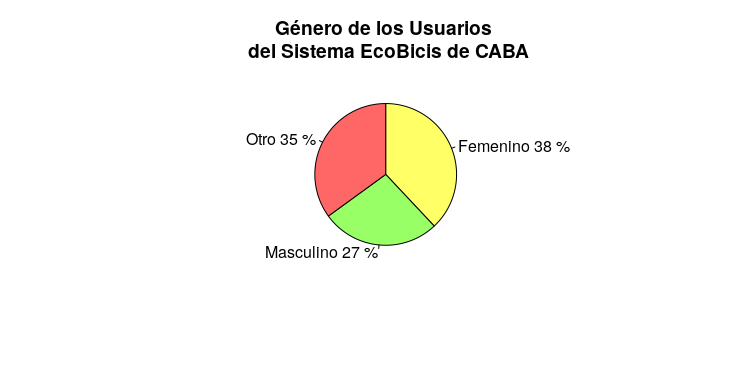
\includegraphics[scale=0.9]{PieChartGenero.png}
  \vspace{-2.5cm}

  De lo descripto se puede observar que las categor\'ias se encuentran bastante uniformemente
  divididas, y que la moda es Femenino, es decir, se cuenta con m\'as usuarios del g\'enero Feminino que de cualquiera de los otros.

  \subsection{Edad de usuario}

  Es importante tener en cuenta que para este an\'alisis univariado se cuenta con un total de 99 usuarios,
  puesto que se debi\'o excluir de los datos recopilados un usuario cuyo valor de Edad se presentaba como faltante.

  Se procedi\'o a la divisi\'on de la variable en intervalos de 5 a\~{n}os de edad,
  quedando su tabla de frecuencias de la siguiente manera: 

    \begin{center}
        \large\textbf{Edad de los Usuarios del 
        Sistema EcoBici de CABA}
    \end{center}

  \begin{myenv}{1}
    \begin{tabularx} {1\textwidth}{ 
        | >{\raggedright\arraybackslash}X 
        | >{\raggedleft\arraybackslash}X 
        | >{\raggedleft\arraybackslash}X 
        | >{\raggedleft\arraybackslash}X 
        | >{\raggedleft\arraybackslash}X |}
       \hline
       \textbf{Edad de usuario} & \textbf{Frecuencia absoluta} & \textbf{Frecuencia relativa} & \textbf{Frecuencia absoluta acumulada} & \textbf{Frecuencia relativa acumulada} \\
       \hline
       [18,23) & 16 & 0.1616 & 16 & 0.1616 \\
       \hline
       [23,28) & 15 & 0.1515 & 31 & 0.3131 \\
       \hline
       [28,33) & 27 & 0.2727 & 58 & 0.5858 \\
       \hline
       [33,38) & 17 & 0.1717 & 75 & 0.7575 \\
       \hline
       [38,43) & 12 & 0.1212 & 87 & 0.8888 \\
       \hline
       [43,48) & 1 & 0.0101 & 88 & 0.8989 \\
       \hline
       [48,53) & 6 & 0.0606 & 94 & 0.9494 \\
       \hline
       [53,58) & 3 & 0.0303 & 97 & 0.9899 \\
       \hline
       [58,63) & 1 & 0.0101 & 98 & 0.9999 \\
       \hline
       [63,68) & 1 & 0.0101 & 99 & 1.0000 \\
       \hline \hline
       \textbf{Total} & 99 & 1.0000 & - & - \\
       \hline
      \end{tabularx}
    \end{myenv}

    \vspace{5mm}

    Manteniendo esta separaci\'on en intervalos se puede visualizar m\'as c\'omodamente esta informaci\'on en un histograma
    que toma como unidad el intervalo de 5 a\~{n}os, as\'i pudiendo presentar la densidad de las \'areas con
    la cantidad de usuarios.

    \hspace{7mm}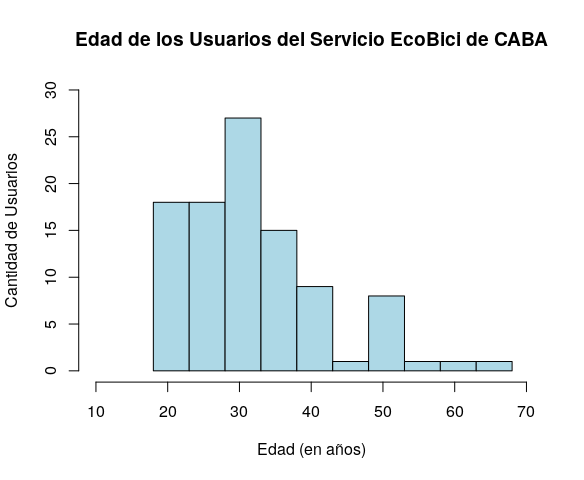
\includegraphics[scale=0.7]{HistEdad.png}

    Acompañando al histograma, tambi\'en resulta \'util la presentaci\'on del pol\'igono de frecuencias (a) y el pol\'igono acumulativo (b).

    \begin{center}
    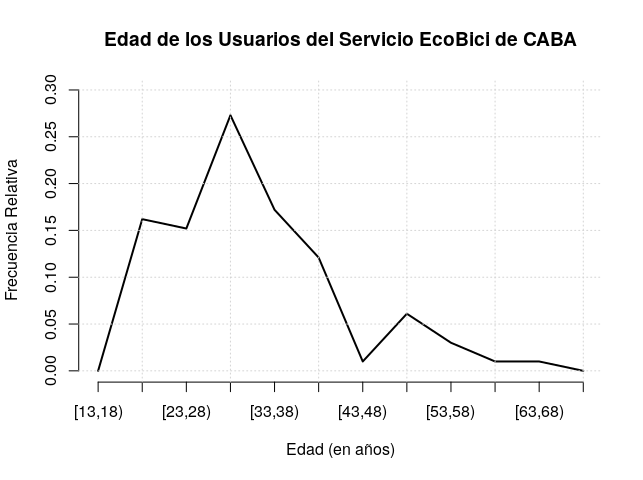
\includegraphics[scale=0.55]{PoligFrecEdad.png}
    \vspace{-4mm}

    (a) Pol\'igono de frecuencias
    \end{center}

    \begin{center}
    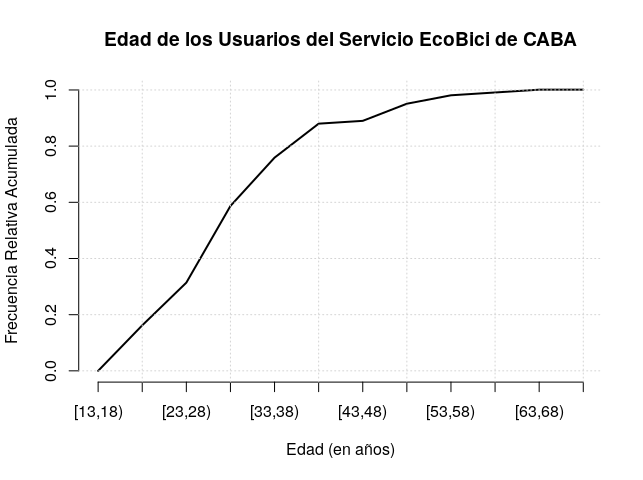
\includegraphics[scale=0.55]{PoligAcumEdad.png}
    \vspace{-4mm}

    (b) Pol\'igono acumulativo
    \end{center}

    Por \'ultimo, dada la condici\'on cuantitativa de la variable edad, resulta interesante hablar sobre sus medidas resumen y respectivas medidas de dispersi\'on. 

    La media es de 32.5100 a\~{n}os con un desv\'io est\'andar de 9.9533 a\~{n}os.

    La mediana la marca la edad de 31 a\~{n}os. El primer cuartil, los 25 a\~{n}os y el tercer cuartil, los 37 a\~{n}os. Por lo tanto, se cuenta con un rango intercuartil de 12 a\~{n}os. 

    La edad m\'inima presentada fue de 19 a\~{n}os y la m\'axima, de 66 a\~{n}os.


  \subsection{D\'ia de recorrido}
  Para dar comienzo al an\'alisis univariado de las variables referidas a los recorridos realizados por los 100 usuarios que 
  comprenden la muestra, resulta pertinente mencionar que se cuenta con un total de 411 recorridos. Este ser\'a referido como tama\~no muestral para estos an\'alisis. 

  La variable D\'ia de recorrido cuenta con 7 categor\'ias: Domingo, Lunes, Martes, Mi\'ercoles, Jueves, Viernes y S\'abado, y su tabla de frecuencia es la que se presenta a continuaci\'on. 

  \begin{center}
    \large\textbf{Recorridos por d\'ia de semana del Sistema EcoBici de CABA}
    
    \begin{tabularx} {0.8\textwidth}{ 
        | >{\raggedright\arraybackslash}X 
        | >{\raggedleft\arraybackslash}X 
        | >{\raggedleft\arraybackslash}X | }
       \hline
       \textbf{D\'ia} & \textbf{Frecuencia absoluta} & \textbf{Frecuencia relativa} \\
       \hline
       Domingo & 63 & 0.1533 \\
       \hline
       Lunes & 63 & 0.1533 \\
       \hline
       Martes & 54 & 0.1314 \\
       \hline
       Mi\'ercoles & 51 & 0.1241 \\
       \hline
       Jueves & 59 & 0.1436 \\
       \hline 
       Viernes & 53 & 0.1290 \\
       \hline 
       S\'abado & 68 & 0.1653 \\
       \hline \hline
       \textbf{Total} & 411 & 1.0000 \\
       \hline
      \end{tabularx}
    \end{center}

    Se puede visualizar mejor esta informaci\'on en el gr\'afico de barras que aparece a continuaci\'on. 

    \hspace{7mm}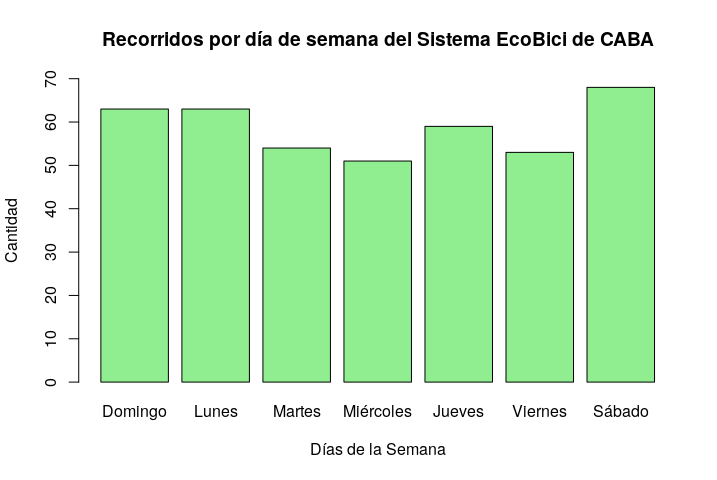
\includegraphics[scale=0.65]{BarPlotDia.png}

    De lo anterior resulta simple notar que la moda de la variable es S\'abado y que la categor\'ia con menor cantidad de recorridos es Mi\'ercoles, aunque, de cualquier manera, las categor\'ias no presentan una gran diferencia entre sus valores.
  
    \subsection{Estaci\'on de origen de recorrido}

    % No agregamos el analisis que tira la funciones de Paretto?

    % 142 estacion de origen
    Tomando en consideraci\'on que se cuenta con 142 estaciones que fueron utilizadas como origen, se decidi\'o presentar dentro del informe un cuadro con las 10 estaciones m\'as utilizadas por la muestra de usuarios. 
    Si se desea obtener el cuadro de frecuencias completo puede acceder a \'el mediante el siguiente enlace {\small \url{https://tablaorigen.000webhostapp.com/origen.html}}.

    Entonces, por un lado, recordando que no se llegan al total esperado de 411 recorridos porque solo presentamos las 10 con mayor frecuencia, se presenta la tabla a continuaci\'on. 

    \begin{center}
      \large\textbf{10 estaciones de EcoBicis de CABA \\
      m\'as frecuentadas como origen}
      
      \begin{tabularx} {1\textwidth}{ 
          | >{\raggedright\arraybackslash}X 
          | >{\raggedleft\arraybackslash}>{\hsize=.5\hsize}X 
          | >{\raggedleft\arraybackslash}>{\hsize=.5\hsize}X | }
         \hline
         \textbf{Estaci\'on} & \textbf{Frecuencia absoluta} & \textbf{Frecuencia relativa} \\
         \hline
         Ramos Mejia, Av Dr Jose Maria Vargas \& Av. Del Libertador & 15 & 0.0365 \\
         \hline
         2292 Montañeses & 13 & 0.0316 \\
         \hline
         3912 Humahuaca & 10 & 0.0243 \\
         \hline
         300 Almafuerte Av. \& Los Patos & 9 & 0.0219 \\
         \hline
         441 Bulnes \& Peron, Juan Domingo, Tte. General & 8 & 0.0195 \\
         \hline
         1785 Espinosa & 7 & 0.0170 \\
         \hline
         3084 Agrelo & 7 & 0.0170 \\
         \hline
         Cordoba 6599 & 7 & 0.0170 \\
         \hline
         Av. Del Libertador, 3260 & 6 & 0.0146 \\
         \hline
         Lavalle \& Acuña De Figueroa, Francisco & 6 & 0.0146 \\
         \hline
      \end{tabularx}
    \end{center}


    Visualizando esta tabla resulta claro que la moda es la estaci\'on ubicada en Ramos Mejia, Av Dr Jose Maria Vargas \& Av. Del Libertador. 

    Sin embargo, por otro lado, teniendo en cuenta la gran cantidad de estaciones se vio como pertinente el recategorizar la variable 
    con respecto a la cantidad de veces que las estaciones fueron utilizadas como origen. Es decir, las categor\'ias nuevas tendr\'an 
    la forma de un n\'umero x que representa la cantidad de recorridos iniciados y su valor asociado ser\'a la cantidad de estaciones 
    que hayan sido origen de una x cantidad de recorridos. 

    % agregue el es decir ...
    Una vez hecha esta recategorizaci\'on se hace f\'acil de reconocer el principio de Paretto que aparece: las categor\'ias con n\'umeros m\'as bajos son las que 
    agrupan la mayor cantidad de estaciones, es decir, la mayor\'ia de las estaciones presentan pocas concurrencias. Esto se puede observar claramente en el siguiente gr\'afico de Paretto. 

    \begin{center}
    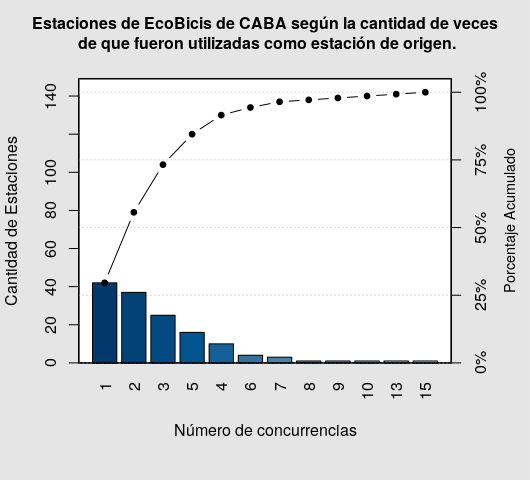
\includegraphics[scale=0.7]{ParettoOrigen.png}
    \end{center}


    \subsection{Estaci\'on de destino de recorrido}

    % 135 estaciones de destino
    Tomando en consideraci\'on que se cuenta con 135 estaciones que fueron utilizadas como destino, se decidi\'o presentar dentro del informe un cuadro con las 10 estaciones m\'as utilizadas por la muestra de usuarios. 
    Si se desea obtener el cuadro de frecuencias completo puede acceder a \'el mediante el siguiente enlace {\small \url{https://tablaorigen.000webhostapp.com/destino.html}} 

    Entonces, por un lado, recordando que no se llegan al total esperado de 411 recorridos porque solo presentamos las 10 con mayor frecuencia, se presenta la tabla a continuaci\'on. 

    \begin{center}
      \large\textbf{10 estaciones de EcoBicis de CABA \\
      m\'as frecuentadas como destino}
      
      \begin{tabularx} {1\textwidth}{ 
          | >{\raggedright\arraybackslash}X 
          | >{\raggedleft\arraybackslash}>{\hsize=.5\hsize}X 
          | >{\raggedleft\arraybackslash}>{\hsize=.5\hsize}X | }
         \hline
         \textbf{Estaci\'on} & \textbf{Frecuencia absoluta} & \textbf{Frecuencia relativa} \\
         \hline
         Lavalle \& Bouchard & 20 & 0.0487 \\
         \hline
         441 Bulnes \& Peron, Juan Domingo, Tte. General & 14 & 0.0341 \\
         \hline
         Amenabar y Mendoza & 14 & 0.0341 \\
         \hline
         Quintino Bocayuva y Don Bosco & 14 & 0.0341 \\
         \hline
         Cevallos, Virrey \& Yrigoyen, Hipolito Av. & 13 & 0.0316 \\
         \hline
         Culpina 121 & 11 & 0.0268 \\
         \hline
         1355 San Martin Av. & 11 & 0.0268 \\
         \hline
         Av. Patricias Argentinas \& Estivao & 8 & 0.0195 \\
         \hline
         3084 Agrelo & 7 & 0.0170 \\
         \hline
         3817 Traful & 7 & 0.0170 \\
         \hline
      \end{tabularx}
    \end{center}


    Visualizando esta tabla resulta claro que la moda es la estaci\'on ubicada en Lavalle \& Bouchard. 

    % cambie algunos origen por destino que estaban mal xd
    
    Sin embargo, por otro lado, teniendo en cuenta la gran cantidad de estaciones y lo realizado con la variable anterior se vio como pertinente el recategorizar la variable 
    con respecto a la cantidad de veces que las estaciones fueron utilizadas como destino. Es decir, las categor\'ias nuevas tendr\'an la forma de un n\'umero x que representa 
    la cantidad de recorridos finalizados y su valor asociado ser\'a la cantidad de estaciones que hayan sido destino de una x cantidad de recorridos. 

    % agregue el es decir ...
    Otra vez, ya hecha esta recategorizaci\'on se hace f\'acil de reconocer el principio de Paretto que aparece: las categor\'ias con n\'umeros m\'as bajos son las que 
    agrupan la mayor cantidad de estaciones, es decir, la mator\'ia de estaciones fueron concurridas pocas veces. Esto se puede observar en el siguiente gr\'afico de Paretto. 

    \begin{center}
      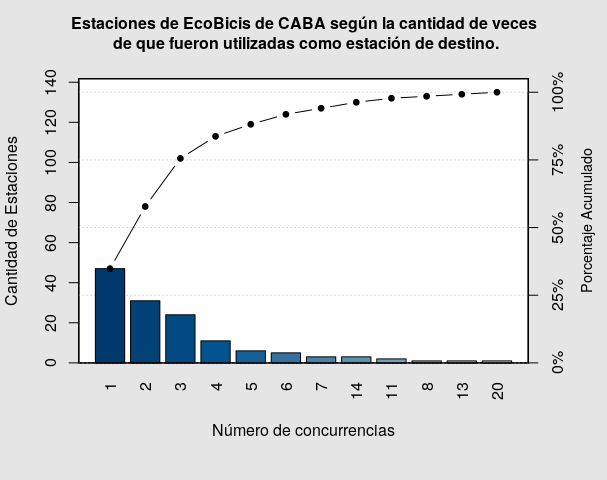
\includegraphics[scale=0.7]{ParettoDest.png}
    \end{center}

    \subsection{Distancia de recorrido}

    Antes de proceder con el an\'alisis resulta importante notar el cambio en la unidad 
    de medida de la distancia respecto a la fuente de los datos. En la fuente las distancias 
    se representan en metros, mientras que en el presente informe se representan en kil\'ometros. 

    Adem\'as, dado que por la continuidad de la variable existen una gran cantidad de valores posibles
    para que tome, se procede a agrupar las categor\'ias de la variable en intervalos de un kil\'ometro. 
    
    Su tabla de frecuencias queda como sigue: 

    \begin{center}
      \large\textbf{Distancia de Recorridos en km \\ del Sistema EcoBici de CABA}
    \end{center}

    \begin{myenv}{1}
      \begin{tabularx} {1\textwidth}{ 
          | >{\raggedright\arraybackslash}X 
          | >{\raggedleft\arraybackslash}X 
          | >{\raggedleft\arraybackslash}X 
          | >{\raggedleft\arraybackslash}X 
          | >{\raggedleft\arraybackslash}X |}
         \hline
         \textbf{Distancia de recorrido} & \textbf{Frecuencia absoluta} & \textbf{Frecuencia relativa} & \textbf{Frecuencia absoluta acumulada} & \textbf{Frecuencia relativa acumulada} \\
         \hline
         [0,1) & 103 & 0.2506 & 103 & 0.2506 \\
         \hline
         [1,2) & 136 & 0.3309 & 239 & 0.5815 \\
         \hline
         [2,3) & 66 & 0.1606 & 305 & 0.7421 \\
         \hline
         [3,4) & 55 & 0.1338 & 360 & 0.8759 \\
         \hline
         [4,5) & 23 & 0.0560 & 383 & 0.9319 \\
         \hline
         [5,6) & 15 & 0.0365 & 398 & 0.9684 \\
         \hline
         [6,7) & 6 & 0.0146 & 404 & 0.9830 \\
         \hline
         [7,8) & 3 & 0.0073 & 407 & 0.9903 \\
         \hline
         [8,9) & 3 & 0.0073 & 410 & 0.9976 \\
         \hline
         [9,10) & 0 & 0.0000 & 410 & 0.9976 \\
         \hline
         [10,11) & 1 & 0.0024 & 411 & 1.0000 \\
         \hline \hline
         \textbf{Total} & 411 & 1.0000 & - & - \\
         \hline
        \end{tabularx}
    \end{myenv}

    Resulta interesante presentar las medidas res\'umenes de la variable y sus respectivas medidas de dispersi\'on.

    \begin{itemize}
      \item La media es de 2.0880 km con un desv\'io est\'andar de 1.7148 km.
      \item El primer cuartil toma el valor de 1.0060 km, mientras que el segundo cuartil (o mediana)
      toma el valor de 1.6130 km y el tercer cuartil, de 3.0390 km.
      \item El rango intercuartil es entonces de 2.0330 km. 
      \item El valor m\'aximo que toma la variable es de 10.9460 km y el m\'inimo es de 0 km (una distancia de recorrido es de 0 km si se devuelve la bicicleta a la misma estaci\'on de donde se la sac\'o).
      \item El intervalo de distancia que cuenta con m\'as recorridos es el [1,2).
    \end{itemize}

    % tal vez se podria explicar que es cada cosa, en el diagrama de paretto tambien, siento que son graficso complejos
    Esta informaci\'on de la variable se puede ver clara y resumida en el siguiente boxplot: 

    \begin{center}
      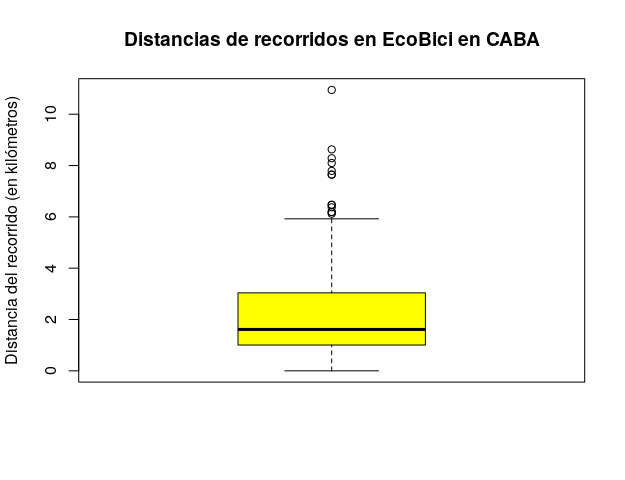
\includegraphics[scale=0.7]{BoxPlotDist.png}
    \end{center}

    \vspace{-1.5cm}

    \subsection{Duraci\'on de recorrido}

    Al igual que con la distancia, previo al an\'alisis de esta variable se debe aclarar
    que se modific\'o la unidad de medici\'on de la variable, pasando de segundos a minutos. 

    % agregue lo de la longitud, esta bien dicho longitud (? xd
    A su vez, tambi\'en por la continuidad de la variable, se decidi\'o dividirla en intervalos de 
    10 minutos hasta llegar a los 132 minutos, donde se agrup\'o a 3 valores muy extremos dentro de un solo intervalo de mayor longitud. 

    \vspace{7mm}

    % ver si no hay que meter un vspace para que quede pegadito al cuadro
    \begin{center}
      \large\textbf{Duraci\'on de Recorridos en minutos \\ del Sistema EcoBici de CABA}
    \end{center}

    \begin{myenv}{1}
      \begin{tabularx} {1\textwidth}{ 
          | >{\raggedright\arraybackslash}X 
          | >{\raggedleft\arraybackslash}X 
          | >{\raggedleft\arraybackslash}X 
          | >{\raggedleft\arraybackslash}X 
          | >{\raggedleft\arraybackslash}X |}
          \hline
          \textbf{Duraci\'on de recorrido} & \textbf{Frecuencia absoluta} & \textbf{Frecuencia relativa} & \textbf{Frecuencia absoluta acumulada} & \textbf{Frecuencia relativa acumulada} \\
          \hline
          (2,12] & 105 & 0.2555 & 105 & 0.2555 \\
          \hline
          (12,22] & 99 & 0.2409 & 204 & 0.4964 \\
          \hline
          (22,32] & 105 & 0.2555 & 309 & 0.7518 \\
          \hline
          (32,42] & 54 & 0.1314 & 363 & 0.8832 \\
          \hline
          (42,52] & 17 & 0.0414 & 380 & 0.9246 \\
          \hline
          (52,62] & 12 & 0.0292 & 392 & 0.9538 \\
          \hline
          (62,72] & 4 & 0.0097 & 396 & 0.9635 \\
          \hline
          (72,82] & 3 & 0.0073 & 399 & 0.9708 \\
          \hline
          (82,92] & 3 & 0.0073 & 402 & 0.9781 \\
          \hline
          (92,102] & 1 & 0.0024 & 403 & 0.9805 \\
          \hline
          (102,112] & 2 & 0.0049 & 405 & 0.9854 \\
          \hline
          (112,122] & 1 & 0.0024 & 406 & 0.9878 \\
          \hline
          (122,132] & 2 & 0.0049 & 408 & 0.9927 \\
          \hline
          (132,485] & 3 & 0.0073 & 411 & 1.0000 \\
          \hline \hline
          \textbf{Total} & 411 & 1.0000 & - & - \\
          \hline
      \end{tabularx}
    \end{myenv}

    \vspace{7mm}

    % agregue lo de los valores
    Se puede ver esta informaci\'on de una forma m\'as clara y ordenada si es presentada en un histograma. 
    Para que este cumpla su prop\'osito de verse as\'i fue necesario excluir del mismo al \'ultimo intervalo 
    que presenta solo 3 recorridos con duraciones muy extremas. Vale aclarar que estos valores son: 191.3000, 267.6500 y  484.5500. 

    Entonces, el nuevo total de recorridos con el que se trabaja es de 408 y este ser\'ia el histograma que representa la duraci\'on de los recorridos (menores a 132 minutos) tomando como unidad los 10 minutos para que as\'i la densidad represente la cantidad de recorridos.

    \begin{center}
      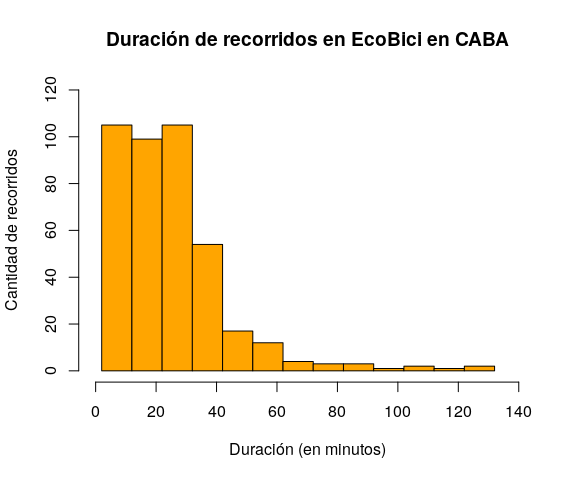
\includegraphics[scale=0.7]{HistDuracion.png}
    \end{center}

    \vspace{-2mm}
    Acompañando al histograma y manteniendo este total de 408 recorridos se presentan el pol\'igono de frecuencias (a) y el pol\'igono acumulativo (b). 

    \begin{center}
      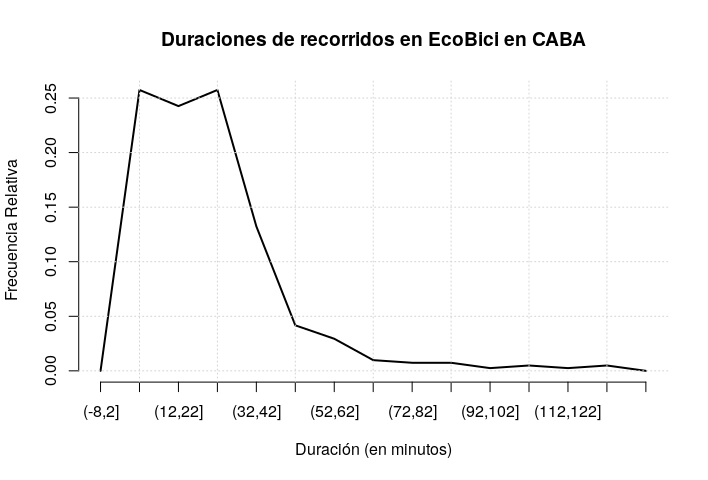
\includegraphics[scale=0.55]{PoligFrecDuracion.png}
      \vspace{-4mm}
  
      (a) Pol\'igono de frecuencias
    \end{center}
  
    \begin{center}
      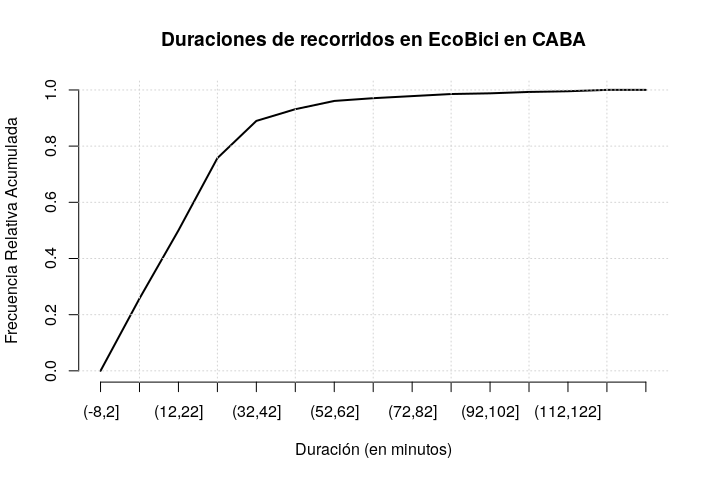
\includegraphics[scale=0.55]{PoligAcumDuracion.png}
      \vspace{-4mm}
  
      (b) Pol\'igono acumulativo
    \end{center}

    Resulta \'util, tambi\'en, el hacer un an\'alisis de las medidas resumen de la variable y sus respectivas medidas de dispersi\'on.
    Para su an\'alisis volvemos a considerar el total de 411 recorridos.

    % che estamos dejando el punto como separador decimal recien aca me di cuenta,,,,,,,,,,,
    La media es de 27.3000 minutos con un desv\'io est\'andar de 32.5626 minutos. 

    En relaci\'on a los cuartiles se puede observar lo siguiente:

    \begin{itemize}
      \item Primer cuartil: 11.6700 minutos.
      \item Segundo cuartil o mediana: 22.4300 minutos.
      \item Tercer cuartil: 31.9100 minutos.
      \item Rango intercuartil: 20.2400 minutos.
    \end{itemize}

    Y, por \'ultimo, el recorrido con mayor duraci\'on fue de 484.5500 minutos y el de menor duraci\'on fue de 2.2000 minutos.

    \section{An\'alisis bivariado}

    \subsection{Duraci\'on de recorrido respecto a D\'ia de recorrido}

    Result\'o interesante combinar las variables D\'ia del recorrido (variable cualitativa) con Duraci\'on del recorrido (variable cuantitativa) para realizar un an\'alisis bivariado. Para ello, se categoriza la duraci\'on del recorrido en intervalos, al igual que se hizo en el an\'alisis univariado. 
    Resulta entonces una tabla con la cantidad (frecuencia absoluta) de recorridos por d\'ia de la semana, de acuerdo a la duraci\'on de los mismos.
     
    \begin{center}
      \large\textbf{Recorridos del Sistema EcoBici de CABA \\
      divididos respecto a Duraci\'on y D\'ia de semana}
    \end{center}

    \begin{myenv}{1}
      \begin{tabularx} {1.15\textwidth}{ 
          | >{\raggedright\arraybackslash}p{55px}
          | >{\raggedleft\arraybackslash}X 
          | >{\raggedleft\arraybackslash}X 
          | >{\raggedleft\arraybackslash}X 
          | >{\raggedleft\arraybackslash}X 
          | >{\raggedleft\arraybackslash}X
          | >{\raggedleft\arraybackslash}X
          | >{\raggedleft\arraybackslash}X 
          | >{\raggedleft\arraybackslash}X |}
          \hline
          \textbf{-} & \textbf{(2,12]} & \textbf{(12,22]} & \textbf{(22,32]} & \textbf{(32,42]} & \textbf{(42,52]} & \textbf{(52,62]} & \textbf{(62,72]} & \textbf{(72,82]} \\
          \hline
          \textbf{Domingo}    & 8 & 17 & 20 & 10 & 4 & 2 & 0 & 0 \\
          \hline
          \textbf{Lunes}      & 14 & 8 & 20 & 8 & 5 & 2 & 1 & 1 \\
          \hline
          \textbf{Martes}     & 20 & 11 & 9 & 7 & 4 & 1 & 0 & 1 \\
          \hline
          \textbf{Mi\'ercoles}  & 17 & 10 & 12 & 7 & 0 & 2 & 1 & 1 \\
          \hline
          \textbf{Jueves}     & 19 & 22 & 10 & 4 & 2 & 2 & 0 & 0 \\
          \hline
          \textbf{Viernes}    & 17 & 18 & 13 & 3 & 0 & 0 & 1 & 0 \\
          \hline
          \textbf{S\'abado}     & 10 & 13 & 21 & 15 & 2 & 3 & 1 & 0 \\
          \hline \hline
          \textbf{Total}        & 105 & 99 & 105 & 54 & 17 & 12 & 4 & 3 \\
          \hline
      \end{tabularx}
    \end{myenv}

    \begin{myenv}{1}
      \begin{tabularx} {1.27\textwidth}{ 
          | >{\raggedright\arraybackslash}p{55px}
          | >{\raggedleft\arraybackslash}X 
          | >{\raggedleft\arraybackslash}X 
          | >{\raggedleft\arraybackslash}X 
          | >{\raggedleft\arraybackslash}X 
          | >{\raggedleft\arraybackslash}X
          | >{\raggedleft\arraybackslash}X
          || >{\raggedleft\arraybackslash}X |}
          \hline
          \textbf{-} & \textbf{(82,92]} & \textbf{(92,102]} & \textbf{(102,112]} & \textbf{(112,122]} & \textbf{(122,132]} & \textbf{(132,485]} & \textbf{Total} \\
          \hline
          \textbf{Domingo}    & 0 & 0 & 1 & 0 & 0 & 1 & 63 \\
          \hline
          \textbf{Lunes}      & 2 & 0 & 1 & 0 & 1 & 0 & 63 \\
          \hline
          \textbf{Martes}     & 0 & 0 & 0 & 0 & 1 & 0 & 54 \\
          \hline
          \textbf{Mi\'ercoles}  & 0 & 0 & 0 & 0 & 0 & 1 & 51 \\
          \hline
          \textbf{Jueves}     & 0 & 0 & 0 & 0 & 0 & 0 & 59 \\
          \hline
          \textbf{Viernes}    & 0 & 0 & 0 & 1 & 0 & 0 & 53 \\
          \hline
          \textbf{S\'abado}     & 1 & 1 & 0 & 0 & 0 & 1 & 68 \\
          \hline \hline
          \textbf{Total}      & 3 & 1 & 2 & 1 & 2 & 3 & - \\
          \hline 
      \end{tabularx}
    \end{myenv}

    \vspace{4mm}

    A fin de visualizar la infromaci\'on de una manera m\'as comprensible, se decidi\'o realizar un boxplot con doble entrada, eliminando los 3 valores m\'as extremos de duraci\'on, que pertencen al \'ultimo intervalo.

    \begin{center}
      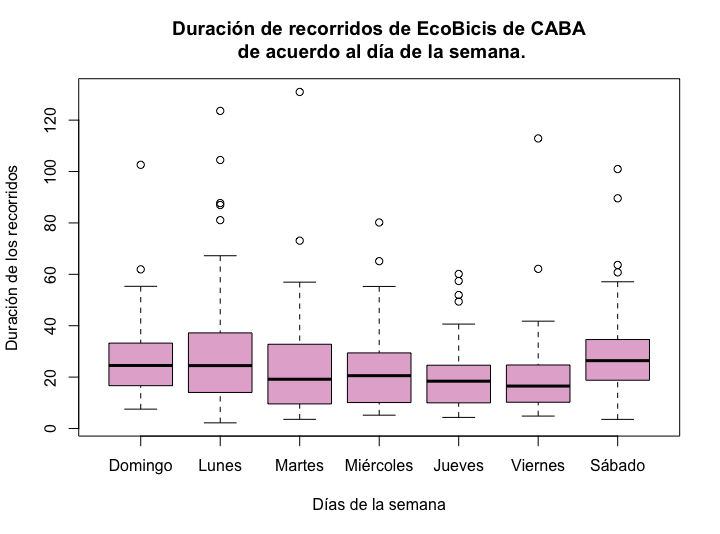
\includegraphics[scale=0.5]{boxplotBivariado.png}
    \end{center}

    Se puede observar que s\'abados y domingos los recorridos tienden a durar m\'as tiempo en general, con dos de los tres valores m\'as extermos siendo d\'ias de fin de semana. %con un promedio de minutos por d\'ia como sigue:

    Adem\'as en el boxplot se visualizan la mediana y los cuartiles y aprovechando la continuidad de la variable, mostramos los promedios de duraci\'on de los recorridos por d\'ia.

    \begin{itemize}
      \item Domingo: 30.7540
      \item Lunes: 30.9802
      \item Martes: 23.9108
      \item Mi\'ercoles: 26.8078
      \item Jueves: 19.9164
      \item Viernes: 20.1981
      \item S\'abado: 35.6978
    \end{itemize}

    \section{Conclusiones}
    Para concluir el presente informe se expone un resumen sobre lo encontrado en los diferentes an\'alisis de variables del Sistema de Ecobici de CABA.

    Repecto al an\'alisis univariado, se puede concluir que: 
    \begin{itemize}
      \item el g\'enero de los usuarios se encuentra dividido muy uniformemente, 
      \item la edad de los mismos var\'ia entre los 19 y 66 años, con la mayor parte de los usuarios teniendo entre 28 y 33 años,
      \item la cantidad de recorridos por d\'ia de semana se encuentra distribuida de manera un tanto uniforme, con la mayor cantidad de recorridos realizados los d\'ias s\'abados
      \item el uso de las estaciones se encuentra dividido de manera bastante desigual, siendo unas pocas las estaciones que reciben la mayor cantidad de recorridos (siendo origen o destino de los mismos),
      \item la distancia de los recorridos var\'ia entre los 0 y 11 kilómetros con la gran mayor\'ia solo llegando a los 3 kil\'ometros, y
      \item la duraci\'on de los recorridos var\'ia entre los 2 y 485 minutos, con la gran mayor\'ia solo llegando a los 32 minutos.
    \end{itemize}
      
    Respecto al an\'alisis bivariado, realizado relacionando el d\'ia de semana con la duraci\'on del recorrido, se puede observar que los fines de semana (s\'abados y domingos) la duraci\'on de los recorridos tiende a ser mayor. Sin embargo, la distribuci\'on es relativamente uniforme.

\end{document}                                                                                  